\chapter{Algorithmique du jeu}

%----------------------------------------------------------------------------------------
%	DÉFINITIONS
%----------------------------------------------------------------------------------------
\section{Définitions}
Les mots que nous allons utiliser pour décrire un objet ou un concept précis mis en oeuvre dans la résolution du problème sont des mots pouvant donner lieu à de nombreuses lectures et approches différentes qui peuvent fausser les démonstrations qui s'appuient dessus. Pour fixer les idées, nous nous devons d'imposer des bases, seul appui pour nos raisonnements ultérieurs.

\label{sect:def}
Une \textit{case} $c$ sera considéré comme une élément admettant une unique couleur (que l'on pourra étiqueter par un entier positif) dans l'ensemble $\Omega$. On admettra pour simplifier que 0 correspond à une abscence de couleur (on dira que la case n'est pas coloriée) et on pourra assimiler cet ensemble à $\mathbb{R}_+$.

Une \textit{grille} $\mathcal{G}$ est une matrice de cases, à laquelle est associée une fonction $\eta_\mathcal{G} : C\rightarrow \Omega$, où $C$ est l'ensemble des cases de la grille et $\forall c\in C, \exists \omega\in \Omega : \eta_\mathcal{G}(c) = \omega$, où $\omega$ est la couleur de la case $c$.

Une case \textit{primaire} est une case qui possède une couleur fixée dans la grille \textit{vide} correspondant à $\mathcal{G}$.

Une case sera dite \textit{remplie} si son état est dans $\Omega^*$.

On définie la notion de \textit{chemin de couleur $\omega$} comme étant une succession de cases de couleur $\omega$ de la grille formant un ensemble 4-connexe. De fait, deux chemins sur la grille ne peuvent pas s'intersecter. Un chemin est \textit{valide} s'il débute dans une case primaire et aboutit dans une autre case primaire.

On appelle cases \textit{adjacentes} deux cases liées par une arrête et qui partagent une couleur commune (deux cases successives sur un chemin associé à une couleur).

%----------------------------------------------------------------------------------------
%	PROBLÈMES
%----------------------------------------------------------------------------------------
\section{Problèmes}
\subsection{Présentation du jeu}
Le jeu Flow consiste à déterminer les chemins valides de chaque couleur dans la grille, et idéalement, à fixer la couleur de chacune des cases. Pour cela, nous devons passer par des étapes de lecture d'une fichier de grille, puis de résolution et enfin d'affichage. Dans cette partie, nous chercherons à présenter les algorithmes principaux utilisées.

\subsection{Spécifications}
Le premier problème auquel nous pouvons nous intéresser est un problème de validation d'une grille remplie (après que l'utilisateur ait joué au jeu par exemple). Le problème est spécifié de la façon suivante :

\begin{verbatim}
Problème : Validation
Entrée : Une grille G remplie.
Sortie : Un booléen indiquant si la grille est valide ou non.
\end{verbatim}

Pour la résolution de ce problème, on doit vérifier les points suivants :
\begin{itemize}
\item pour chaque couleur, l'ensemble des cases de cette couleur doit être connexe,
\item les cases d'une même couleur forment un chemin sans boucles,
\item ce chemin débute dans une case primaire pour aboutir dans une autre case primaire.
\end{itemize}

Comme à chaque case est associée une unique couleur, on interdit ici toute intersection non-vide entre les ensemble de différentes couleurs.

Le second problème que nous avons traité est le problème d'existence ou non d'une solution, spécifié de la façon suivante :

\begin{verbatim}
Problème : Resolution
Entrée : Une grille G.
Sortie : Une grille R et un booléen r tel que :
    r = FAUX s'il n'existe pas de solutions de G,
    r = VRAI si R est une solution de G.
\end{verbatim}

\subsection{Algorithmes}
\subsubsection{Validation}
La fonction principale du moteur de jeu est la vérification d'une grille résolue. En effet le moteur graphique gère la jouablilité d'un coup, ce qui enlève des possibilités de coups et réduit la complexité de la vérification. \\

	Par exemple, une grille où des sommets colorés non primaires non relié à des sommets primaires n'est pas une grille que nous pouvons obtenir avec notre moteur graphique. \\

L'algorithme fonctionne de la façon suivante : \\
\begin{algorithm}[H]
 \KwData{Graphe représentant la grille}
 \KwResult{Booléen Vrai si la grille est bien remplie, Faux sinon}
 
 \While{Toutes les couleurs n'ont pas été testées}{
  Choisir nouvelle couleur\;
  Chercher sommet primaire correspondant\;
  Stocker l'indice de ce sommet\;
  	\While{Sommet courant n'est pas primaire de clé différente de celle stockée}{
		\eIf{Sommet courant est primaire de même clé}{
				retourner Faux\;
		}	
		{
				Passer au sommet voisin\;
		}

	}
		
  retourner Vrai\;
}
\caption{Vérification de grille}
\end{algorithm}

	Dans notre implémentation, le degré de chaque sommet est limité à deux. Lorsque deux sommets sont adjacents sur la grille, de la même couleur mais non liés, le parcours se fera correctement.\\
    
    De plus, chaque sommet coloré étant lié à un sommet primaire, les seuls cas où l'algorithme retournera faux sont lorsque la grille n'est pas complétement remplie, ou lorsque qu'un chemin n'atteint pas un sommet primaire distinct. Nos listes d'adjacences se remplissent en tête, lorsqu'un sommet est au bout d'un chemin, il n'a qu'un seul voisin. En fait, l'algorithme retournera en arrière et parcourera le même chemin une seconde fois. Il se stoppera en arrivant sur un sommet primaire de même clé que celui de départ.

L'algorithme de validation a été construit avec l'interface graphique utilisant la librairie \textit{ltk}. L'utilisateur lorsqu'il joue au jeu ne peux pas effectuer certaines actions, comme relier deux cases de couleurs différentes, intersecter des chemins, etc. Par conséquent, la difficulté de notre fonction de validation se retrouve transférée à la gestion de l'interface graphique elle-même, et nous avons ainsi une fonction de valisation qui n'effectue que des vérifications de base pour valider un remplissage.

\subsubsection{Résolution}
Notre algorithme de résolution s'inspire de la recherche en profondeur dans un graphe (DFS). Son principe consiste à construire récursivement les chemins reliant les couleurs de la grille en appelant à chaque étape une recherche en profondeur qui tient compte des modifications apportés.

Considérons la grille de jeu représentée sur la Figure~\vref{subfig:start}. Avant de décrire le déroulement de l'algorithme sur cette grille nous allons mettre au point un certain nombre de conventions utiles pour la suite. Premièrement, à chaque couleur nous attribuons les entiers suivants (Rouge:1, Orange:2, Jaune:3, Bleu:4, Vert:5).

Deuxièmement, si l'algorithme est amené à choisir une direction où se déplacer, il devra la choisir selon l'ordre suivant : nord, est, sud, ouest. Ces conventions sont totalement arbitraires, néanmoins elles servent à prendre des décisions pendant l'éxéution des instructions. Finalement, nous appellerons obstacle les bords de la grille ou un noeud de couleur différentes de la couleur recherchée.\\

A l'état initial, le solver choisit la première couleur à relier, celle correspondant à l'entier le plus faible (Rouge). Ensuite, il en détermine une position dans la grille et choisit une direction disponible pour se déplacer (nord). Puis, il se déplace en ligne droite  suivant cette direction jusqu'à rencontrer un obstacle (bords de la grille) (cf. Figure~\vref{subfig:p1}).

Arrivé à cet étape, le solver doit encore décider d'une direction vers laquelle il va tourner (est) (cf. Figure~\vref{subfig:p2}). Si aucune direction n'est disponible, le solver retourne en arrière d'une case jusqu'à en trouver une. Ce processus est répeté jusqu'à ce que le solver tombe sur un noeud primaire ayant la même couleur à relier et différent du noeud de départ. Les Figures~\vref{subfig:p4} et ~\vref{subfig:p3} correspondent à des états intermédiares, on y voit notamment le solveur changer de direction lorsqu'il ne trouve aucune issue. La Figue ~\vref{subfig:p5} correspond à la fin de la recherche pour la couleur rouge.

La prochaine étape va consister à relier la deuxième couleur d'entier le plus faible (Orange). Toujours en suivant les même règles de recherche, nous constatons qu'au bout de quelques déplacements le chemin rouge bloque le chemin orange (cf. Figure~\vref{subfig:p6}), le solveur fait donc des retours en arrière, ce qui le conduit en fin de compte à retracer un nouveau chemin pour la couleur rouge (cf. Figure~\vref{subfig:p7}). Cette fois-çi la voie est libre pour le chemin orange qui peut se déplacer vers l'est (cf. Figure~\vref{subfig:p8}). Le solveur va continuer ainsi à appliquer les mêmes règles jusqu'à relier toutes les couleurs dans l'ordre croissant des entiers qui leurs sont attribués (cf. Figure~\vref{subfig:p9}).\\

A partir de cette description, nous pouvons constater que l'algorithme est amené à plusieurs reprises à prendre des décisions influancant ses déplacements. Ses décisions concernent notamment, le choix de la couleur, le choix de la direction, le déplacement en ligne droite et le retour en arrière. L'algorithme doit aussi identifier quelques situations particulières : aucun déplacement possible, obstacle atteint, couleur reliée.

\begin{figure}[h]
  \centering
  \begin{subfigure}[b]{0.3\textwidth}
      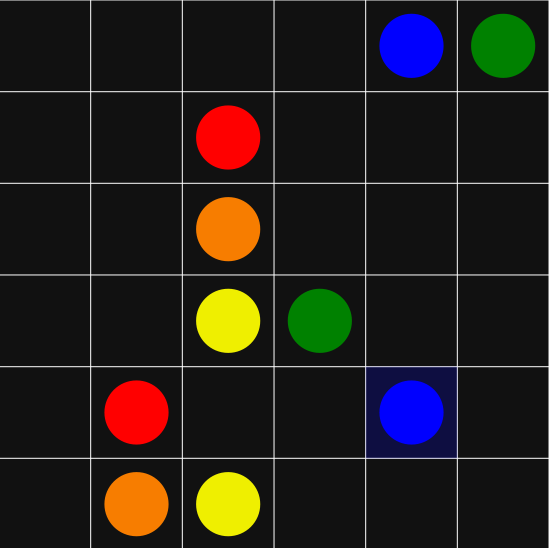
\includegraphics[width=\linewidth]{start.png}
      \caption{Grille de départ}
      \label{subfig:start}
   \end{subfigure}
   \begin{subfigure}[b]{0.3\textwidth}
      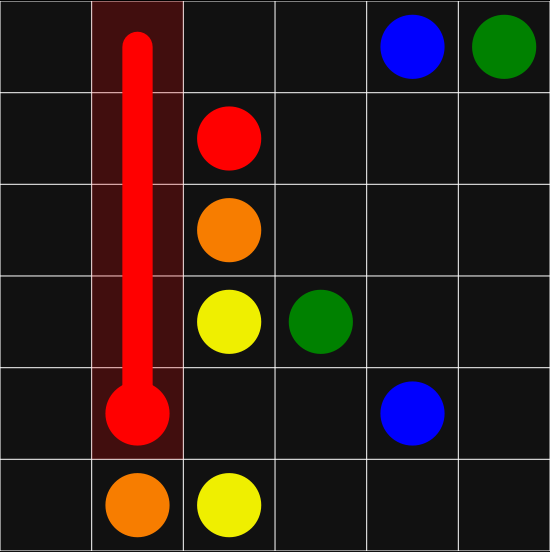
\includegraphics[width=\linewidth]{p1.png}
      \caption{Obstacle trouvé}
      \label{subfig:p1}
   \end{subfigure}
   \begin{subfigure}[b]{0.3\textwidth}
      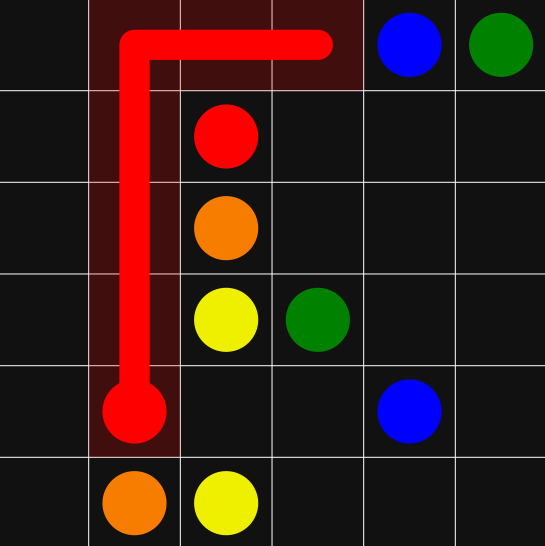
\includegraphics[width=\linewidth]{p2.png}
      \caption{Aller vers l'Est}
      \label{subfig:p2}
   \end{subfigure}
   \begin{subfigure}[b]{0.3\textwidth}
      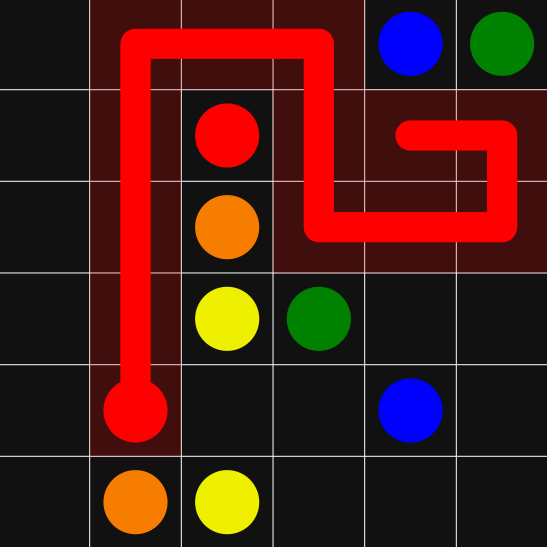
\includegraphics[width=\linewidth]{p4.png}
      \caption{Aucune issue}
      \label{subfig:p4}
   \end{subfigure}
   \begin{subfigure}[b]{0.3\textwidth}
      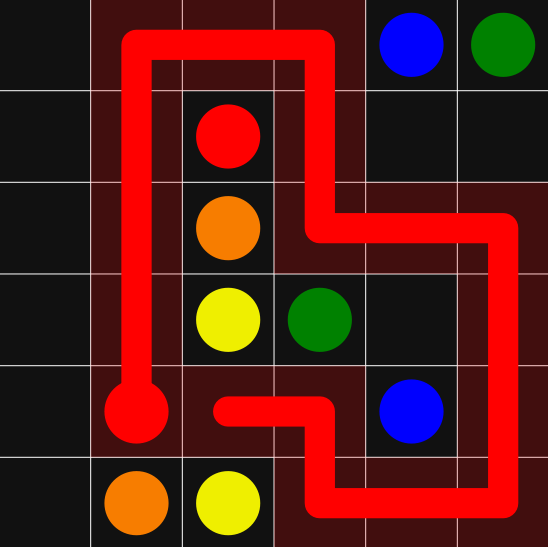
\includegraphics[width=\linewidth]{p3.png}
      \caption{Aucune issue}
      \label{subfig:p3}
   \end{subfigure}
   \begin{subfigure}[b]{0.3\textwidth}
      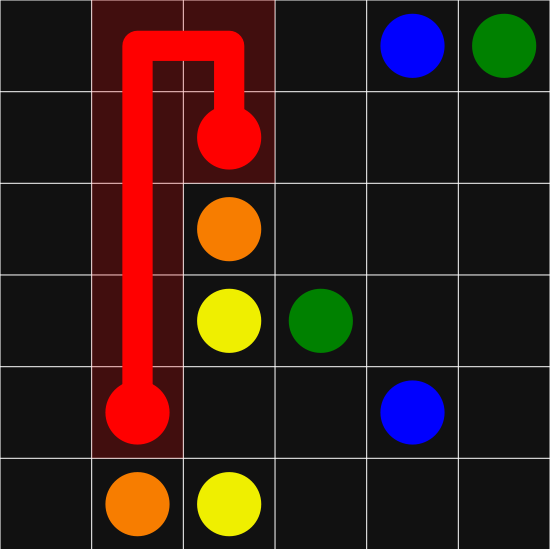
\includegraphics[width=\linewidth]{p5.png}
      \caption{Couleur reliée}
      \label{subfig:p5}
   \end{subfigure}
   \begin{subfigure}[b]{0.3\textwidth}
      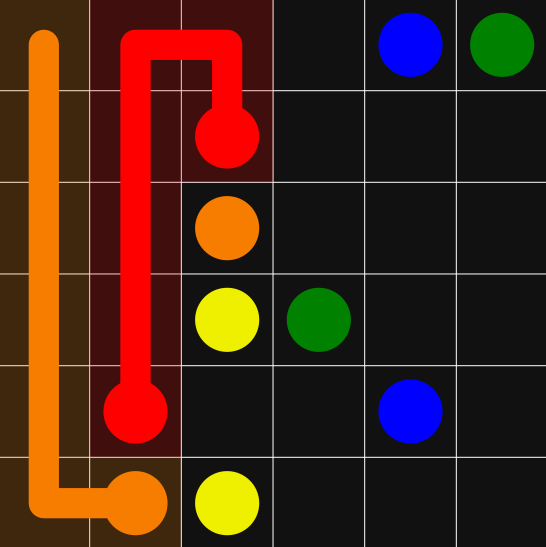
\includegraphics[width=\linewidth]{p6.png}
      \caption{Orange bloqué}
      \label{subfig:p6}
   \end{subfigure}
   \begin{subfigure}[b]{0.3\textwidth}
      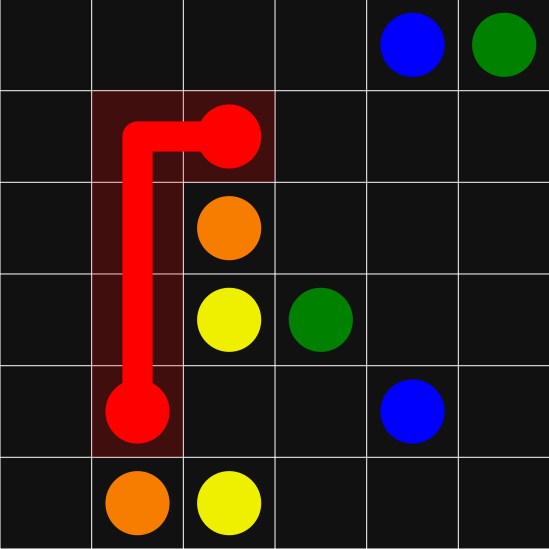
\includegraphics[width=\linewidth]{p7.png}
      \caption{Rouge rectifié}
      \label{subfig:p7}
   \end{subfigure}
   \begin{subfigure}[b]{0.3\textwidth}
      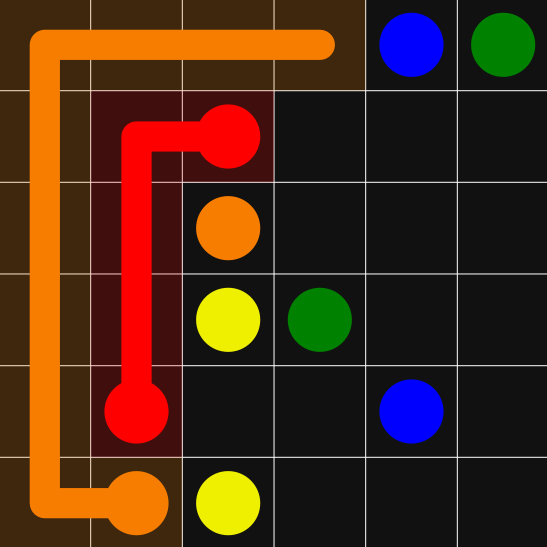
\includegraphics[width=\linewidth]{p8.png}
      \caption{Orange libre}
      \label{subfig:p8}
   \end{subfigure}
   \begin{subfigure}[b]{0.3\textwidth}
      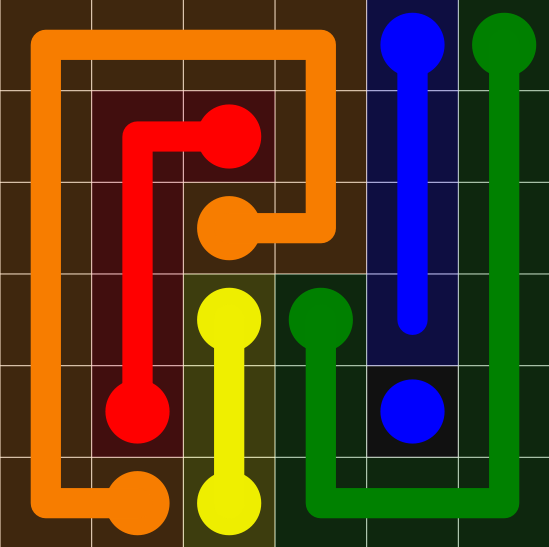
\includegraphics[width=\linewidth]{p9.png}
      \caption{Dernière étape}
      \label{subfig:p9}
   \end{subfigure}
   \label{fig:etapes}
   \caption{Étapes de résolution}
\end{figure}

